\documentclass[11pt]{article}

\usepackage[utf8]{inputenc}
\usepackage{graphicx}
\usepackage{amsmath, amssymb, geometry, cancel}
\usepackage{pgfplots,pgfplotstable}
\usepackage{float}
\usepackage{parskip}
\usepackage{tikz,tikz-3dplot,xcolor}
\usetikzlibrary{optics}
\usetikzlibrary{arrows.meta}
\usetikzlibrary{calc,shapes.geometric}
\usepackage{listings}
\usepackage{mathrsfs}
\usepackage[scr=rsfs]{mathalfa}
\usepackage{mhchem}
\usepackage{svg}
\usepackage{caption}
\usepackage{subcaption}
 \geometry{
 a4paper,
 total={170mm,257mm},
 left=15mm,
 right=15mm,
 top=10mm, 
 }
\newcommand{\E}[2]{E^{#1}_{#2}}
\newcommand{\tform}[2]{{\Lambda^{#1}}_{#2}}
\newcommand{\krist}[2]{{\Gamma^{#1}}_{#2}}
\newcommand{\pfrac}[2]{\dfrac{\partial #1}{\partial #2}}
\newcommand{\curl}[1]{\nabla \times \mathbf{#1}}
\renewcommand{\div}[1]{\nabla \cdot \mathbf{#1}}
\newcommand{\grad}[1]{\nabla \mathbf{#1}}
\newcommand{\infint}[1]{\int_{-\infty}^\infty #1}
\renewcommand{\bf}[1]{\mathbf{#1}}
\renewcommand{\cal}[1]{\mathcal{#1}}
\newcommand{\sinc}{\mbox{sinc}}
\newcommand{\lf}{\left}
\newcommand{\rt}{\right}
\newcommand{\mbf}{\mathbf}

\title{N-Body modelling}
\author{Fergus Babb: ID 20229006}
\date{}
\newpage






\begin{document}
\maketitle

\begin{figure}[H]
  \centering
	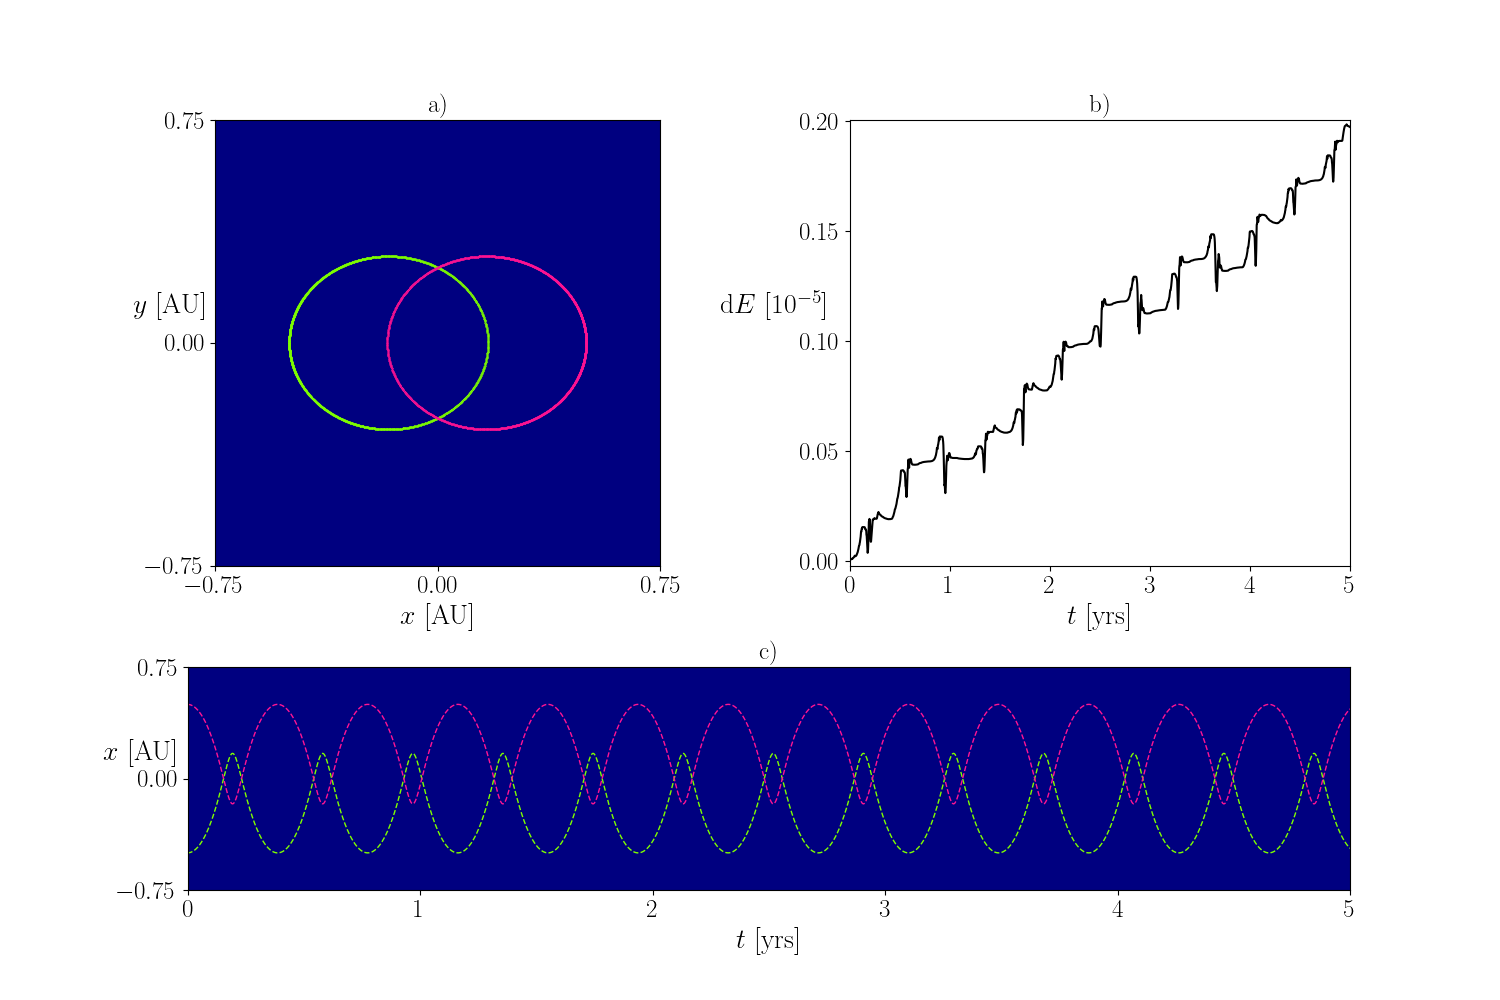
\includegraphics[scale=.45]{Validation_fig.png}
\caption{Results from the required validation test, showing two masses with $M_1=M_1=M_\odot$ orbiting each other for $5$ years with initial conditions given by $x_{1,2}=\mp 0.5$[AU], $v_{x1,x2} = 0$[m/s]$, v_{y1,y2} = \pm 15000$[m/s]. a) shows the dynamics for all time steps, plotted as a function of $x$ and $y$ in units of [AU]. c) shows the $x$ coordinate as a function of time (in years), together with a. these plots agree with the validation test. As an additional test, the differential change in energy was plotted, b) shows this. After 5 years it can be seen that the total energy of the system increases by a factor of $\approx 2.0\times 10^{-4}\%$, which is well within reasonable bounds, suggesting that for this system the automatic tolerance in the solver used is valid. \\
For the full dynamics see \texttt{Validation.gif}.}
\label{Val_fig}
\end{figure}
\newpage


\begin{figure}[H]
\centering
    \subfloat[A recreation of the evolution in Burrau's problem.]{\label{Bur_plots}\includegraphics[scale=.5]{Burrau_plots.png}} \\
    \subfloat[Energy deviations corresponding to the evolution in \ref{Bur_plots}.]{\label{Bur_energy}\includegraphics[scale=.6]{Burrau_energy.png}}
    \caption{This figure shows the extension to 3 bodies via Burrau's well documented test in which at the vertices of a pythagorean $345$ triangle, masses of the same ratios, with $0$ initial velocity are allowed to evolve. In \ref{Bur_plots}, the $x$ and $y$ axes display unit lengths $L$, and $t$ is unit time, defined by allowing $T^2GM/L^3=1$ with $M=M_\odot, L=$ AU and $G$ being Newton's gravitational constant, giving $T\approx 0.159$[yrs], dimensionless time $t=\tau/T$ where $\tau$ is real time. Using one five-thousandth of the standard integration tolerance, with $\approx 10^7$ total steps these plots well reproduce the findings of V.Szebehely and C.F.Peters [1], up to the final time steps of plot vi., where the deviation is very small, but given the chaotic behaviour, would lead to greater differences for later times. It can be seen once again from \ref{Bur_energy} that the energy is being conserved to within a negligible uncertainty of $\approx 10^{-5}\%$, which is to be expected given the more stringent tolerances, compared to the verification case. The spikes at $t \approx 2, 9, 15, 30$ are due to extreme close encounters. For the full dynamics see \texttt{Burraus$\_$test.gif}.} 
    \label{Bur_tes}
\end{figure}
\newpage


\begin{figure}[H]
\centering
\begin{subfigure}{.45\textwidth}
	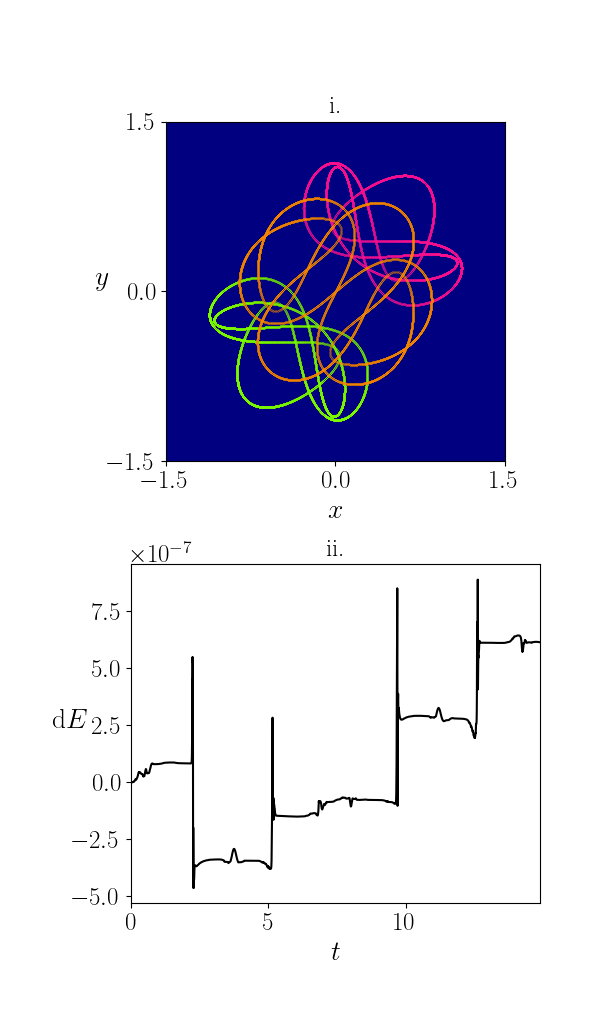
\includegraphics[scale=.45, trim={0cm, 0cm, 0cm, 3cm}]{Moth_hightol.png}
\caption{Known periodic 'MOTH-III' solution for 3 equal\\ mass bodies with automatic integration tolerance.}
\label{Moth_hightol}
\end{subfigure}%
\centering
\begin{subfigure}{.45\textwidth}
	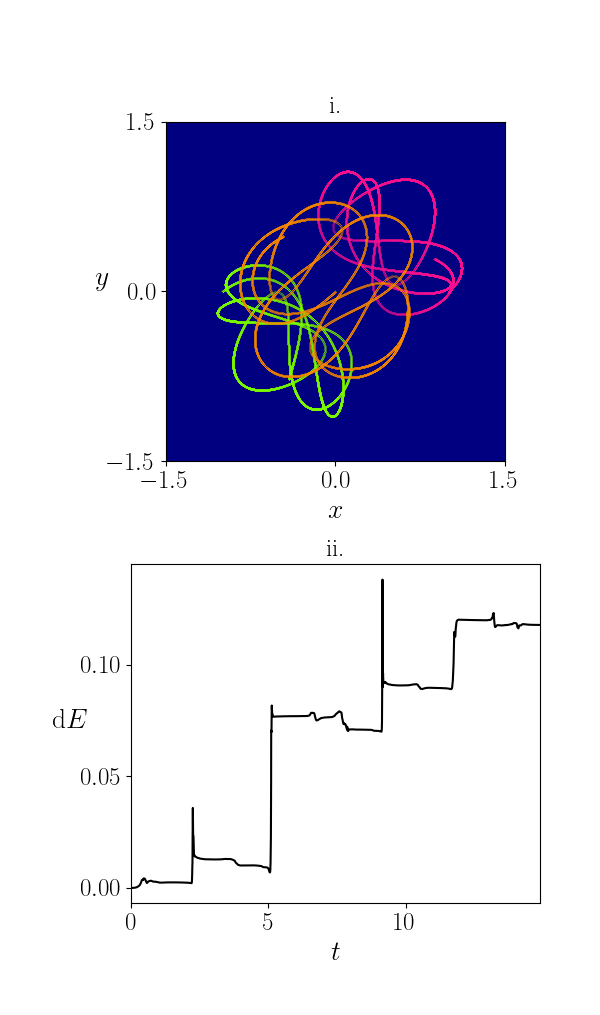
\includegraphics[scale=.45, trim={0cm, 0cm, 0cm, 1cm}]{Moth_medtol.png}
\caption{Integration tolerances increased to $10^5$ the standard value.}
\label{Moth_medtol}
\end{subfigure}\\
\centering
\begin{subfigure}{.45\textwidth}
	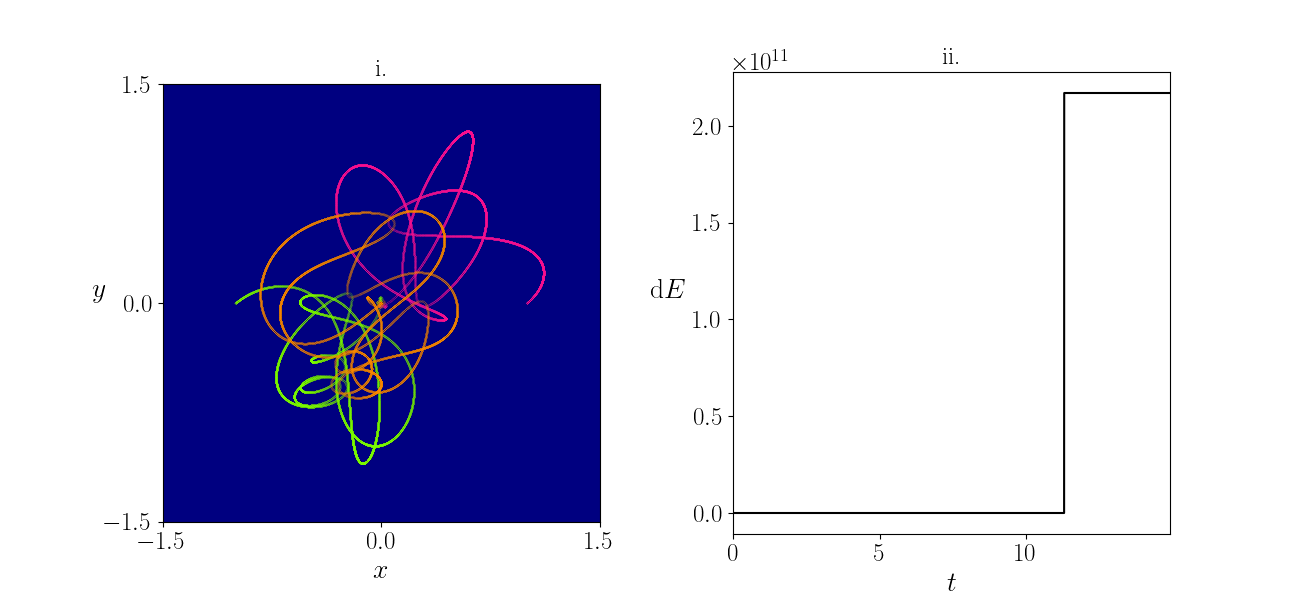
\includegraphics[scale=.45, trim={8cm, 1cm, 1cm, 0cm}]{Moth_lowtol.png}
\caption{Integration tolerances increased to $10^6$ the standard value.}
  \label{Moth_lowtol}
\end{subfigure}
\caption{Using a known periodic solution 'MOTH-III' to demonstrate the need for integration tolerances in chaotic systems. [2] found MOTH-III to be periodic for approximately 22 periods using a $25^{\mbox{th}}$ order TSM (Taylor series method). The findings in \ref{Moth_hightol} only consider the first oscillation period, however it is unnecessary to go further as the demonstration here is to only show the short term behaviour, which agrees with the periodicity as found previously. By increasing the tolerances by a factor of $10^{5}$, the chaotic behaviour begins to arise; given the relative stability of MOTH-III, quite a large step was needed to show this eventual chaos. Note here how the energy differential has increased $\sim 10^5$-fold. Finally, by increasing the tolerances by only another $\times 10$, the chaos can very much be seen, and given this is only for one 'period', this shows that for particularly unstable systems, or long term behaviours, as in \ref{Bur_tes}, much higher tolerances are necessary for the simulation to be valid. It can also be seen that the energy is definitely no longer conserved, as the differential has increased by a further $\sim 10^{10}$ for only a $\times 10$ increase in the tolerance. For the full dynamics, the ability to change tolerances yourself, and to look at other known solutions such as GOGGLES and YIN-YANG-III, please see the relevant included folder.}
\label{MOTH-III}
\end{figure}
\newpage

\begin{figure}[H]
  \centering
	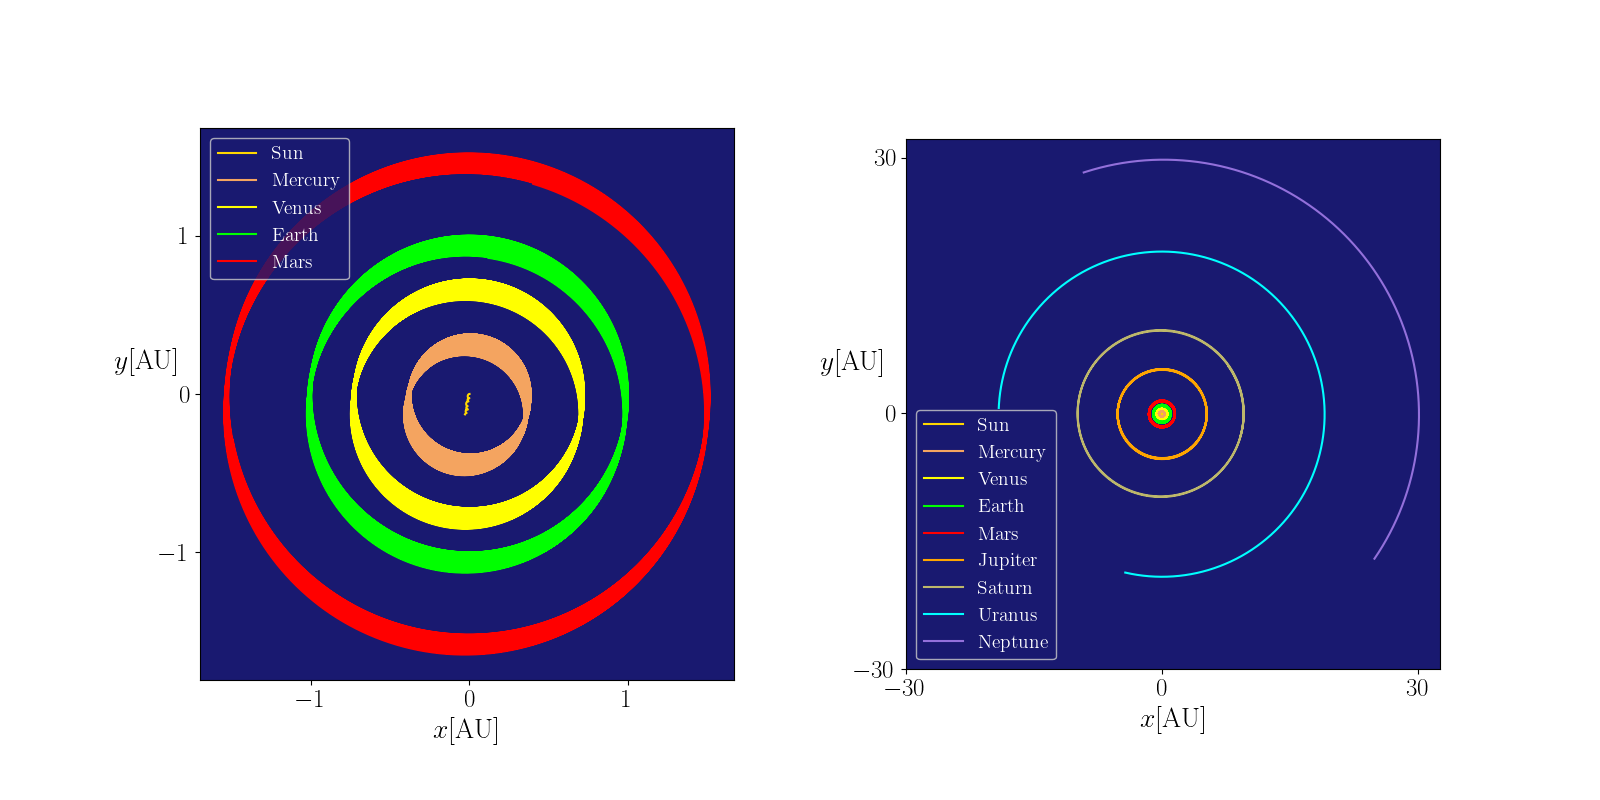
\includegraphics[scale=.45]{Solar_syst_fig.png}
\caption{This figure shows the evolution of the planets and sun in our solar system in a period of $65$ years. Notice how the inner planets, which orbit $>50$ times each, compared to the outer gas giants which orbit less than $3$ times each. This can be seen in that the terrestrial planets and the Sun move a lot, whereas the outer planets are so far out that they don't feel this inner oscillation and so appear more stable. This could be improved with higher tolerances and more precise initial conditions, as well as increasing to 3D to implement eccentricity.\\
For the full dynamics see \texttt{Solar$\_$system.gif}.}
    \label{Solar_syst}
\end{figure}
\newpage





\begin{figure}[H]
\centering
	\includegraphics[scale=.45]{Single cluster.png}
\caption{The full evolution for 10 $\sim$ solar masses with $0.1M_{\odot} \le M \le 100M_{\odot}$ around a larger mass (non relativistic black hole) with mass $1000M_{\odot}$, shown in white. The masses follow a random distribution governed by the relatively well accepted initial mass distribution of number of stars in certain mass range $\propto M^{-1.2}$ [3]. While this is hard to interpret, this is made easier by showing the initial positions with a thick cross. It can be seen that generally, the lighter masses are bound much closer to the central mass, or if they start with sufficient velocity (deternimed with a random distribution favouring a clockwise orbit, and inversely proportional to mass, by equating potential energy from distance to central mass with kinetic energy and thus a velocity), they are released to infinity. The larger masses, with smaller initial velocities are much more likely to be bound to the central mass. For the full dynamics, which will give a much clearer representation of the results, please see \texttt{10Bodies$\_$singlecluster.gif}.}
\label{SingleClust}
\end{figure}
\newpage


\begin{figure}[H]
\centering
	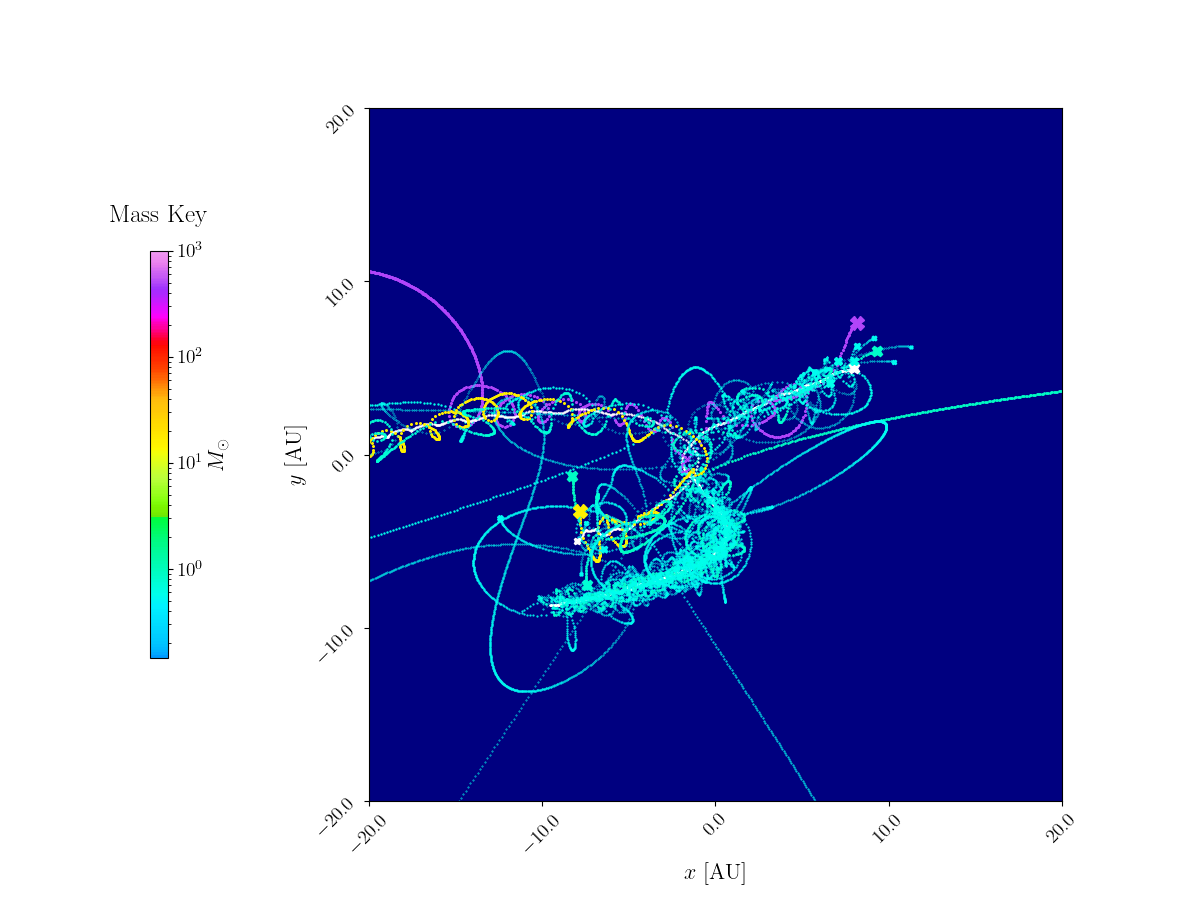
\includegraphics[scale=.45]{Merger.png}
\caption{The full evolution for a merger of two clusters similar to that in \ref{SingleClust}. Here the central masses are now $1000M_{\odot}$ and $500M_{\odot}$, again shown in white, with the larger cluster consisting of $3/5$ of the total particles. It can be seen that once again, initially, the heavier masses are bound to their host mass, whereas the lighter masses are either tightly bound or are expelled completely, save a minority of cases. When these clusters merge we see initially an 'explosion' of the particles, particularly the lighter masses, as more energy is required to slingshot the larger masses. At later times we see the heavier central mass holding on to a large proportion of the bound small masses, whereas the lighter central mass continues, with the heavier masses bound to it (Note the yellow mass being transferred from the heavier cluster to the lighter one, and the lilac mass remaining bound to the lighter mass). In conclusion, this simulation shows that in general, a merger of two star clusters under gravitational influence, will result in either a complete expulsion of particles, which will recombine at larger time scales, two smaller clusters, one bearing the majority of the massive particles, the other most of the lighter particles, or they will combine completely, but this can only happen if one of the central masses isn't slingshot away by the other. In other words, the late time dynamics depend on how the massive central objects interact, effectively because the orbiting masses are almost negligible. For the full dynamics of this figure see \texttt{20Bodies$\_$merger.gif}.}
\label{SingleClust}
\end{figure}

\section{References}
\begin{enumerate}
\item Szebehely, V. and Peters, C.F., 1967. Complete solution of a general problem of three bodies. The Astronomical Journal, 72, p.876.
\item Li, X. and Liao, S., 2014. On the stability of the three classes of Newtonian three-body planar periodic orbits. Science China Physics, Mechanics \& Astronomy, 57(11), pp.2121-2126.
\item Kroupa, P. and Jerabkova, T., 2021. The initial mass function of stars and the star-formation rates of galaxies. Star-Formation Rates of Galaxies, 55.
\end{enumerate}






\end{document}
